% \appendix
\chapter{Función sigmoide}\label{sec:sigmoide} %% TODO: pasar a anexos
            Esta función ha sido introducida en la Ecuación(\ref{eq:sigmoide}) y representa, históricamente, la función 
            más utilizada en las primeras redes neuronales artificiales porque modela de manera aproximada, una respuesta 
            característica de las neuronas del cerebro \cite{narayan1997generalized}, pero sobre todo, porque posee las dos características mencionadas 
            anteriormente: naturaleza no lineal y diferenciable. Otra característica llamativa, es que se puede interpretar 
            a la salida como una función de probabilidad, pues sus valores van desde $0$ a $1$, como se puede apreciar 
            en la Figura(\ref{fig:sigmoide}). Usualmente se incluye un parámetro adicional para controlar el \textit{radio de activación}
            que hace que la función responda con más o menos sensibilidad a su entrada.

            \begin{figure}[!h] 
                \centering
                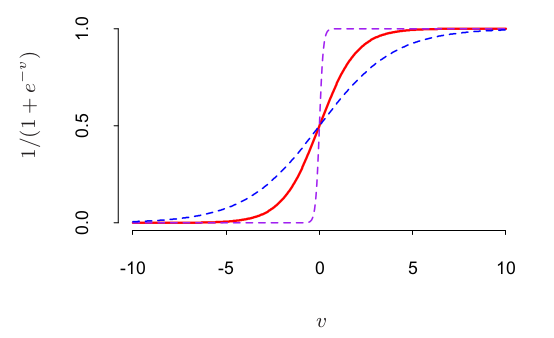
\includegraphics[width=0.75\textwidth]{img/sigmoide}
                \caption[Gráfico de la función sigmoide]{Gráfico de la función sigmoide $\sigma(v) = 1 / (1 + e^{(-v)})$ (curva roja), y dos variaciones con un radio de activación de la forma $\sigma(sv)$ con valores $s=1/2$ (curva azul) y $s=10$ (curva púrpura) . Fuente: \cite{Goodfellow-et-al-2016} }
                \label{fig:sigmoide}
            \end{figure}
            
            Pese a las características anteriormente mencionadas, la función sigmoide tiene una gran desventaja: el llamado 
            \textit{desvanecimiendo de gradientes} \cite{hochreiter1998vanishing}. Este fenómeno ocurre cuando la activación 
            de una capa oculta tiene valores muy altos o muy negativos, se puede apreciar en la Figura(\ref{fig:sigmoide}), que 
            para estos valores, la derivada tiene un valor muy pequeño, aproximándose a cero mientras más grandes sean los valores.
            Este fenómeno ocasiona que, mientras se realiza la retropropagación de gradientes, dado que el gradiente tiene un valor 
            muy bajo, el ajuste en los pesos sea mínimo, deteniendo así el aprendizaje de la neurona en la que ocurre el fenómeno.

            Esta dificultad se presenta especialmente cuando la red neuronal se compone de varias capas ocultas y 
            ha motivado el desarrollo de nuevas funciones de activación que no presenten esta limitación y puedan 
            mantener valores de gradientes adecuados durante el entrenamiento.
            
            Cabe resaltar que, pese a las dificultades con la propagación de los gradientes de la función sigmoide, ésta se suele 
            utilizar bastante en la capa de salida, cuando se trata de clasificación binaria, ya que representa de manera adecuada
            la noción de probabilidad, lo cual es deseable en este tipo de modelos.